\section{Ros2ForUnity}
\label{ros2forunity}

Ros2ForUnity es una librería de Unity que permite crear nodos de ROS 2 con código C\# de Unity.


\subsection{Instalación de Ros2ForUnity}
Para instalar la librería se han seguido los documentos markdown del repositorio de GitHub del proyecto \footnote{Ros2ForUnity Windows Installation: \url{https://github.com/RobotecAI/ros2-for-unity/blob/develop/README-WINDOWS.md}}. En este proyecto se ha comprobado su funcionamiento hasta el commit:

\begin{verbatim}
3f548920bc4c33e178707a888d01592905bef1e9
\end{verbatim}



Hay que prestar especial atención a los prerequisitos y a los avisos importantes que se señalizan dentro del ``README-WINDOWS.md'' del repositorio. Y en ejecutar la Powershell en modo administrador.



Al momento de construir el proyecto Ros2ForUnity, es necesario seleccionar la versión ``overlay''. Esta elección se debe a que la versión ``standalone'' proporciona una instancia única de ROS dentro de Unity, que no corresponde al comportamiento deseado para este proyecto.



Ahora hay dos opciones para instalar el asset en Unity. Ejecutar el comando siguiente para crear un package e instalarlo en Unity de manera habitual:

\begin{verbatim}
create\_unity\_package.ps1
\end{verbatim}

O copiar y pegar en los assets del proyecto de Unity el directorio que se encuentra en \textbf{install/asset/}.

\subsection{Uso de Ros2ForUnity con ROS2}

Una vez instalado Ros2ForUnity en Unity, es importante recordar que se debe iniciar Unity a través de la terminal después de iniciar ROS2. Esto se debe a que Ros2ForUnity necesita acceso a la instancia de ROS2 que se ejecuta en el sistema para funcionar correctamente.

Primero, se debe iniciar ROS2. Si estás utilizando ROS2 Humble en Windows, puedes hacerlo ejecutando el siguiente comando en PowerShell:

\begin{verbatim}
C:\dev\ros2_humble\local_setup.ps1
\end{verbatim}

Asegúrate de que tu terminal esté en el directorio que contiene tu script de configuración de ROS2 local antes de ejecutar este comando.

Después de haber iniciado ROS2, puedes abrir tu proyecto de Unity a través de la terminal utilizando el comando unity con la opción -projectPath seguido de la ruta a tu proyecto:

\begin{verbatim}
unity.exe -projectPath "D:\Unity\Unity Projects\Thesis-Unity-Pan-Tilt"
\end{verbatim}

Con ROS2 en funcionamiento y Unity abierto de esta manera, deberías ser capaz de utilizar Ros2ForUnity para crear nodos de ROS2 con el código C\# de Unity.


\subsection{Consideraciones}

Es necesario asignar a la variable de entorno ROS\_IP una dirección IP que permita la comunicación entre ROS2 en la WSL y ROS2 en el sistema operativo Windows.

\begin{figure}[!htb]
    \centering
    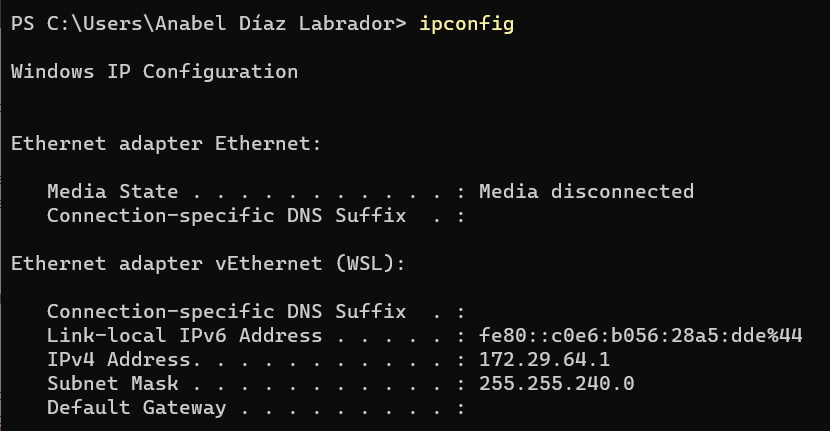
\includegraphics[width=0.8\linewidth]{figures/wsl-network-powershell.png}
    \caption{Red de la WSL visualizada en PowerShell}
    \label{figure:wsl-network-powershell}
\end{figure}



La necesidad de usar la dirección IP de la WSL se origina del hecho de que la comunicación entre la WSL y Windows se realiza a través de una red virtual interna. Esta dirección IP asegura que los mensajes enviados por ROS2 en la WSL sean recibidos por ROS2 en Windows y viceversa. Se puede observar en la figura \ref{figure:wsl-network-powershell}.



Comandos para asignar la dirección IP:



En Windows (usando PowerShell):
\begin{verbatim}
$env:ROS_IP='172.29.67.184'
\end{verbatim}


En WSL:
\begin{verbatim}
export ROS_IP=172.29.67.184
\end{verbatim}